\documentclass[11pt]{article}

\usepackage[letterpaper,top=1in,bottom=1in,left=1.25in,right=1.25in]{geometry}
\usepackage{setspace}
\usepackage[parfill]{parskip}
\usepackage{hyperref}
\usepackage{enumitem}
\usepackage{tikz,ifthen,xstring,calc,pgfkeys,pgfopts}
\usepackage{tikz-uml}
\usepackage{float}

\tikzumlset{fill class=black!15}

\begin{document}

\begin{figure}

  \begin{center}
    \begin{tikzpicture}

      \umlclass[x=2, y=10, width=15ex]{ComponentVisitor}{
      }{
        \umlvirt{visitTetrisPiece(TetrisPiece\&) : void} \\
        \umlvirt{visitTetrisBoard(TetrisBoard\&) : void} \\
        \umlvirt{visitPanel(Panel\&) : void}
      }

      \umlclass[x=2, y=6, width=15ex]{TetrisVisitor}{
      }{
        visitTetrisPiece(TetrisPiece\&) : void \\
        visitTetrisBoard(TetrisBoard\&) : void \\
        visitPanel(Panel\&) : void
      }

      \umlinherit{TetrisVisitor}{ComponentVisitor}


    \end{tikzpicture}
  \end{center}

  \caption{TetrisVisitor architecture}

\end{figure}


\begin{figure}

  \begin{center}
    \begin{tikzpicture}


      \umlclass[x=2, y=0, width=15ex]{TetrisComponent}{
      }{
        \umlvirt{accept(ComponentVisitor\& visitor) : void}
      }
      
      \umlclass[x=2, y=-7, width=15ex]{TetrisPiece}{
      }{
        accept(ComponentVisitor\& visitor) : void \\
        \{ \\
        \hspace{0.3cm} visitor.visitTetrisPiece( *this ); \\
        \}
      }

      \umlclass[x=-2, y=-4, width=15ex]{TetrisBoard}{
      }{
        accept(ComponentVisitor\& visitor) : void
      }

      \umlclass[x=6, y=-4, width=15ex]{Panel}{
      }{
        accept(ComponentVisitor\& visitor) : void 
      }


      \umlinherit{TetrisPiece}{TetrisComponent}
      \umlinherit[geometry=|-|]{TetrisBoard}{TetrisComponent}
      \umlinherit[geometry=|-|]{Panel}{TetrisComponent}

    \end{tikzpicture}
  \end{center}

  \caption{TetrisComponent architecture}

\end{figure}

\end{document}
